\section{Βελτιστοποίηση Ακολουθίας Επίσκεψης των Δωματίων}
\label{section:room_sequence_implementation}

Tο επόμενο βήμα της μελέτης αυτής είναι ο υπολογισμός της βέλτιστης σειράς επίσκεψης των δωματίων από το ρομποτικό όχημα. Μετρική βελτίωσης της διαδρομής αποτελεί η συνολική απόσταση που χρειάζεται να διανύσει το όχημα. Το πρόβλημα αυτό αποτελεί το γνωστό \emph{πρόβλημα του περιπλανώμενου πωλητή - TSP}. Η προσέγγιση που προτείνεται χρησιμοποιεί δύο παραλλαγές του Hill Climbing αλγόριθμου που ονομάζονται \emph{RRHC} και \emph{anneal HC}, η σύγκριση των οποίων θα πραγματοποιηθεί μέσω των πειραμάτων. Επιπλέον, για τον γρήγορο υπολογισμό των αποστάσεων ανάμεσα σε όλες τις πόρτες δημιουργείται ο αντίστοιχος γράφους του χώρου. Τέλος, είναι χρήσιμο να υπολογιστεί η πόρτα εισόδου και η πόρτα εξόδου για κάθε δωμάτιο σύμφωνα με την διαδρομή που έχει βρεθεί, κάτι που θα φανεί περισσότερο στην επόμενη ενότητα. Η διαδικασία, λοιπόν, αποτελείται από τα παρακάτω βήματα:

\begin{itemize}
    \setlength\itemsep{-0.2em}
    \item δημιουργία γράφου με κόμβους τις πόρτες του χάρτη
    \item υπολογισμός όλων των αποστάσεων
    \item υπολογισμός βέλτιστης διαδρομής
    \item αντιστοιχία αλληλουχίας πορτών με αλληλουχία δωματίων
    \item υπολογισμός πόρτας εισόδου και εξόδου για κάθε δωμάτιο δεδομένης της διαδρομής που βρέθηκε
\end{itemize}


\subsection{Δημιουργία Γράφου Δωματίων}
\label{subsection:room_graph}

Αρχικά, λοιπόν, δημιουργείται ένας γράφος, με σκοπό τον ακριβή υπολογισμό των αποστάσεων μεταξύ όλων των πορτών. Η χρήση του ενισχύει την ταχύτητα και την ακρίβεια της διαδικασίας. Ο χώρος μπορεί κάλιστα να προσεγγιστεί από έναν γράφο με την μορφή που αναλύεται στη συνέχεια. Οι κόμβοι πόρτας που έχουν υπολογιστεί αποτελούν τους κόμβους του γράφου, οι αποστάσεις τους αποτελούν τα βάρη των ακμών ενώ συνδεδεμένοι είναι οι κόμβοι που ανήκουν στο ίδιο δωμάτιο. Οι αποστάσεις μεταξύ των γειτονικών κόμβων υπολογίζονται με τη χρήση brushfire με αρχή το ένα σημείο και πέρας το δεύτερο \ref{alg:point_to_point_brushfire}, προσεγγίζοντας έτσι την πραγματική απόσταση μεταξύ τους στον ελεύθερο χώρο. Αντίθετα, για τους μη γειτονικούς κόμβους χρησιμοποιείται ο αλγόριθμος Dijkstra \ref{alg:dijkstra} για κάθε συνδιασμό κόμβων. Με τον τρόπο αυτό υπολογίζεται μια ικανοποιητικά ακριβής απόσταση μεταξύ όλων των κόμβων πόρτας του χώρου, ενώ αποφεύγεται η χρήση ευκλείδιων αποστάσεων που χάνουν σημαντικά σε ακρίβεια και η χρήση brushfire μεταξύ όλων των κόμβων που απαιτεί μεγαλύτερο χρόνο εκτέλεσης.



\begin{algorithm}[!htb]
\caption{Point to Point Brushfire}
\label{alg:point_to_point_brushfire}
\begin{algorithmic}[1]
    \Function{pointToPointBrushfire}{start, finish, ogm}
    \State $brushfire = np.zeros(ogm.shape)$
    \State $brushfire[ogm > 49] = 1$
    \State $brushfire[ogm == -1] = 1$
    \State $brushfire[start] = 2$
    \State $brushfire[finish] = -1$
    \State $step = 2$
    \State $changed = 1$
    \State $iters\_made = 0$
    \State $found = 0$
    \While{$changed == 1$ and not $found$}
        \State $changed = 0$
        \For{$i$ = 1 to ($brushfire.width$ - 1)}
            \For{$j$ = 1 to ($brushfire.height$ - 1)}
                \If{$brushfire[i][j] <= 0$ and a neighbor's brushfire value is equal to step}
                    \If{$brushfire[i][j] == -1$}
                        \State $found = 1$
                    \EndIf
                    \State $brushfire[i][j] = step + 1$
                    \State $changed = 1$
                \EndIf
            \EndFor
        \EndFor
        \State $step += 1$
        \State $iters\_made += 1$
    \EndWhile
    \If{$brushfire[finish] <= 0$}
        \State $iters\_made = -1$
    \EndIf
    \State \Return $iters\_made$
\end{algorithmic}
\end{algorithm}


Η δημιουργία του γράφου βασίζεται στην ήδη υλοποιημένη δομή Dijkstar \cite{dijkstar}. Αυτή περιέχει κώδικα γραμμένο σε \emph{Python} με μεθόδους που δίνουν τη δυνατότητα εύκολης δημιουργίας ενός γράφου και εκτέλεσης του αλγορίθμου Dijkstra σ' αυτόν. Όπως φαίνεται και στον \ref{alg:compute_door_distances} γίνεται χρήση των παρακάτω μεθόδων της δομής Dijkstar.

\begin{itemize}
    \setlength\itemsep{-0.2em}
    \item $Graph()$: κατασκευαστής (constructor) της κλάσης του γράφου
    \item $add\_edge(node\_1, node\_2, weight)$: μέθοδος δημιουργίας ακμής στον γράφο μεταξύ δύο σημείων και με βάρος ίσο με $weight$ 
    \item $find\_path(graph, node\_1, node\_2)$: μέθοδος υπολογισμού το συντομότερου μονοπατιού μεταξύ δύο κόμβων του γράφου με τον αλγόριθμο Dijkstra
\end{itemize}

Υπολογίζονται τελικά οι αποστάσεις κάθε σημείου ως προς κάθε άλλο και αποθηκεύονται σε έναν διδιάστατο πίνακα. Επιπλέον, ο αλγόριθμος επιστρέφει και την δημιουργημένη δομή του γράφου, ώστε να μπορεί να αξιοποιηθεί και στα επόμενα τμήματα της διαδικασίας.



\begin{algorithm}[H]
\caption{Compute Door Distances}
\label{alg:compute_door_distances}
\begin{algorithmic}[1]
    \Function{computeDoorDistances}{door\_nodes, room\_doors}
    \State $graph = Graph()$
    \Comment{Create graph}
    \For{$room$ in $room\_doors$}
        \If{$len(room) > 1$}
            \For{$i$ in $range(len(room))$}
                \For{$j$ in $range(i+1, len(room))$}
                    \State $node\_id\_1 = door\_nodes.index(room[i])$
                    \State $node\_id\_2 = door\_nodes.index(room[j])$
                    \State $dist = pointToPointBrushfire(room[i], room[j], ogm)$
                    \If{$dist < 0$}
                        \State \Return
                    \EndIf
                    \State $graph.add\_edge(node\_id\_1, node\_id\_2, dist)$
                    \State $graph.add\_edge(node\_id\_2, node\_id\_1, dist)$
                \EndFor
            \EndFor
        \EndIf
    \EndFor
    \State \Comment{Calculate graph's distances between all nodes}
    \State $doors\_length = len(door\_nodes)$
    \If{$doors\_length >= 2$}
        \State $distances = np.zeros((doors\_length, doors\_length))$
        \For{$i$ in $range(doors\_length)$}
            \For{$j$ in $range(i+1, doors\_length)$}
                \State $\_, \_, \_, dist = find\_path(graph, i, j)$
                \State $distances[i][j] = dist$
                \State $distances[j][i] = distances[i][j]$
            \EndFor
        \EndFor
     \Else
        \State $distances[0][0] = 0$
    \EndIf
    \State \Return $distances, graph$
\end{algorithmic}
\end{algorithm}


Δύο παραδείγματα δημιουργίας του εν λόγω γράφου πάνω στο OGM παρουσιάζονται στα σχήματα \ref{fig:graph_on_map_examples}. Με μπλε έχουν σημειωθεί όλες οι πόρτες κάθε περιβάλλοντος, ενώ οι συνδεδεμένοι κόμβοι, δηλαδή οι κόμβοι που ανήκουν στο ίδιο δωμάτιο, έχουν ενωθεί με κόκκινη γραμμή.

\begin{figure}[h]
     \centering
     \captionsetup{justification=centering}
     \begin{subfigure}[b]{0.5\textwidth}
         \centering
         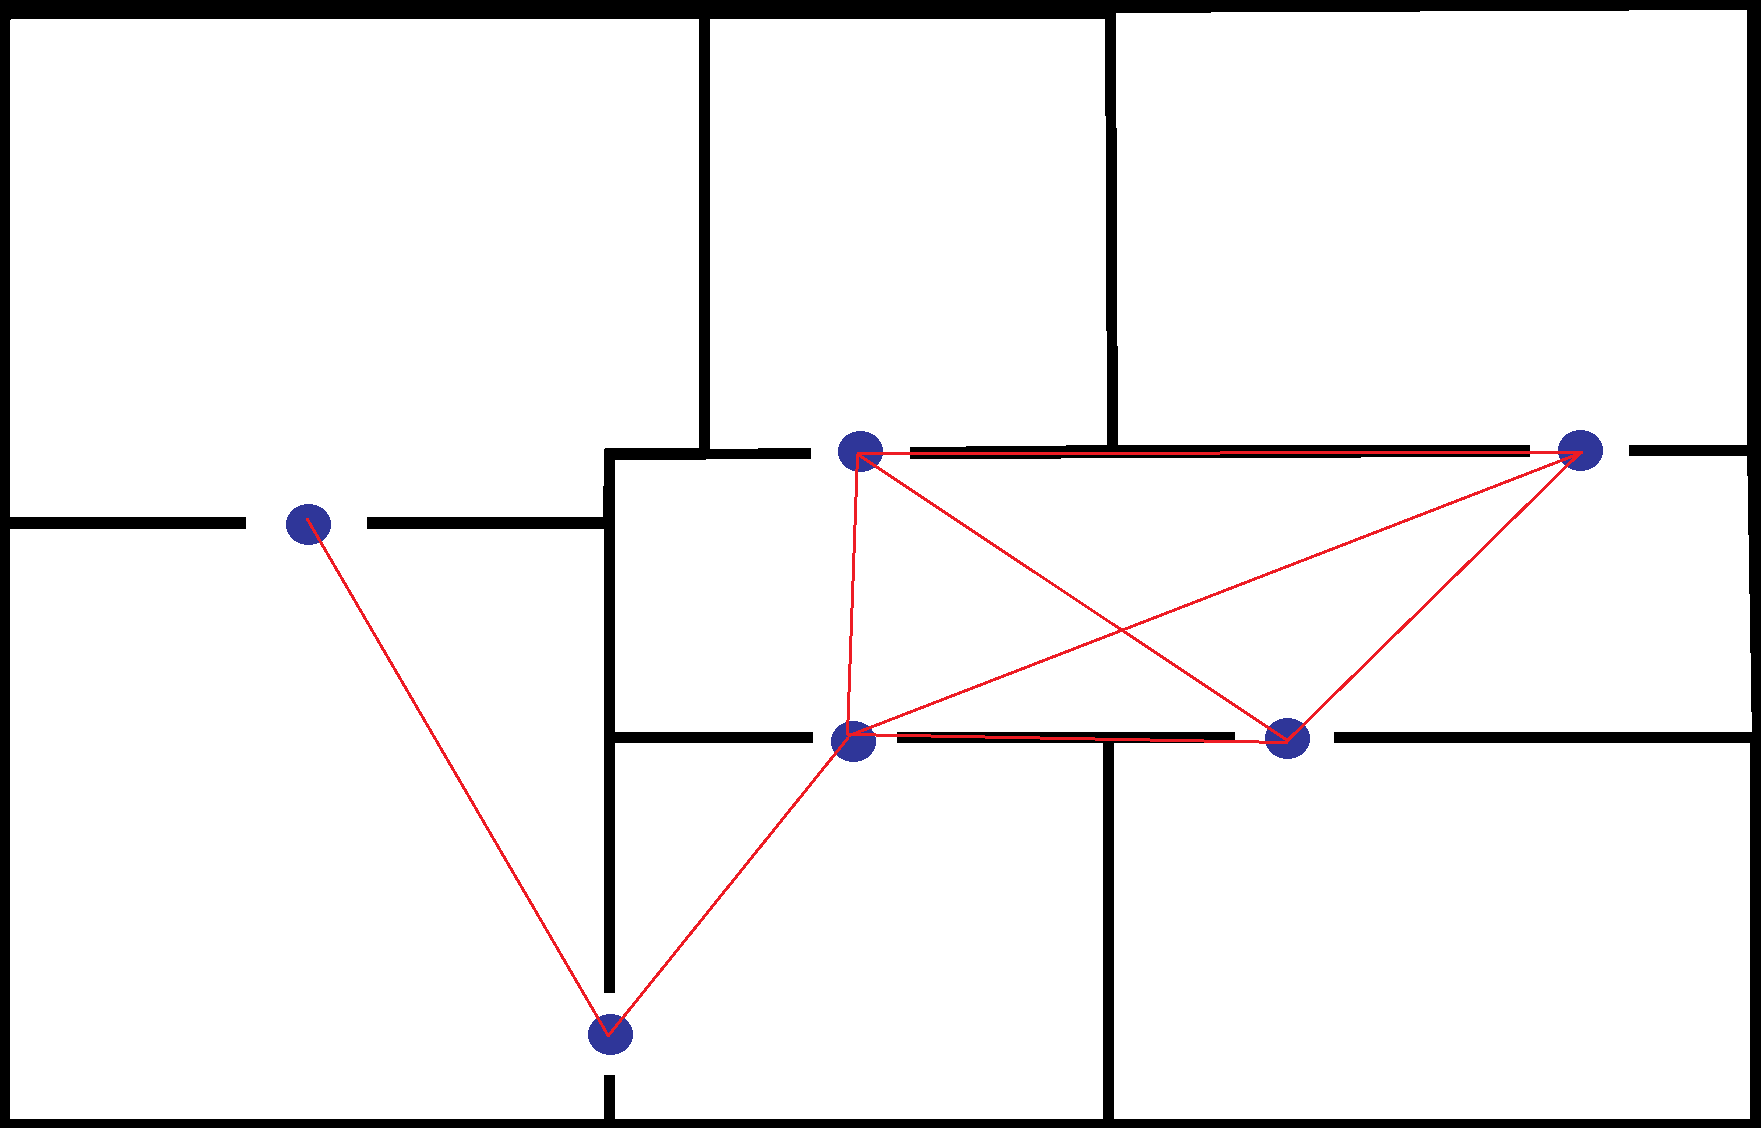
\includegraphics[width=0.8\textwidth]{./images/chapter5/graph_on_map_1.png}
         \label{fig:graph_on_map_1}
     \end{subfigure}%
     \begin{subfigure}[b]{0.5\textwidth}
         \centering
         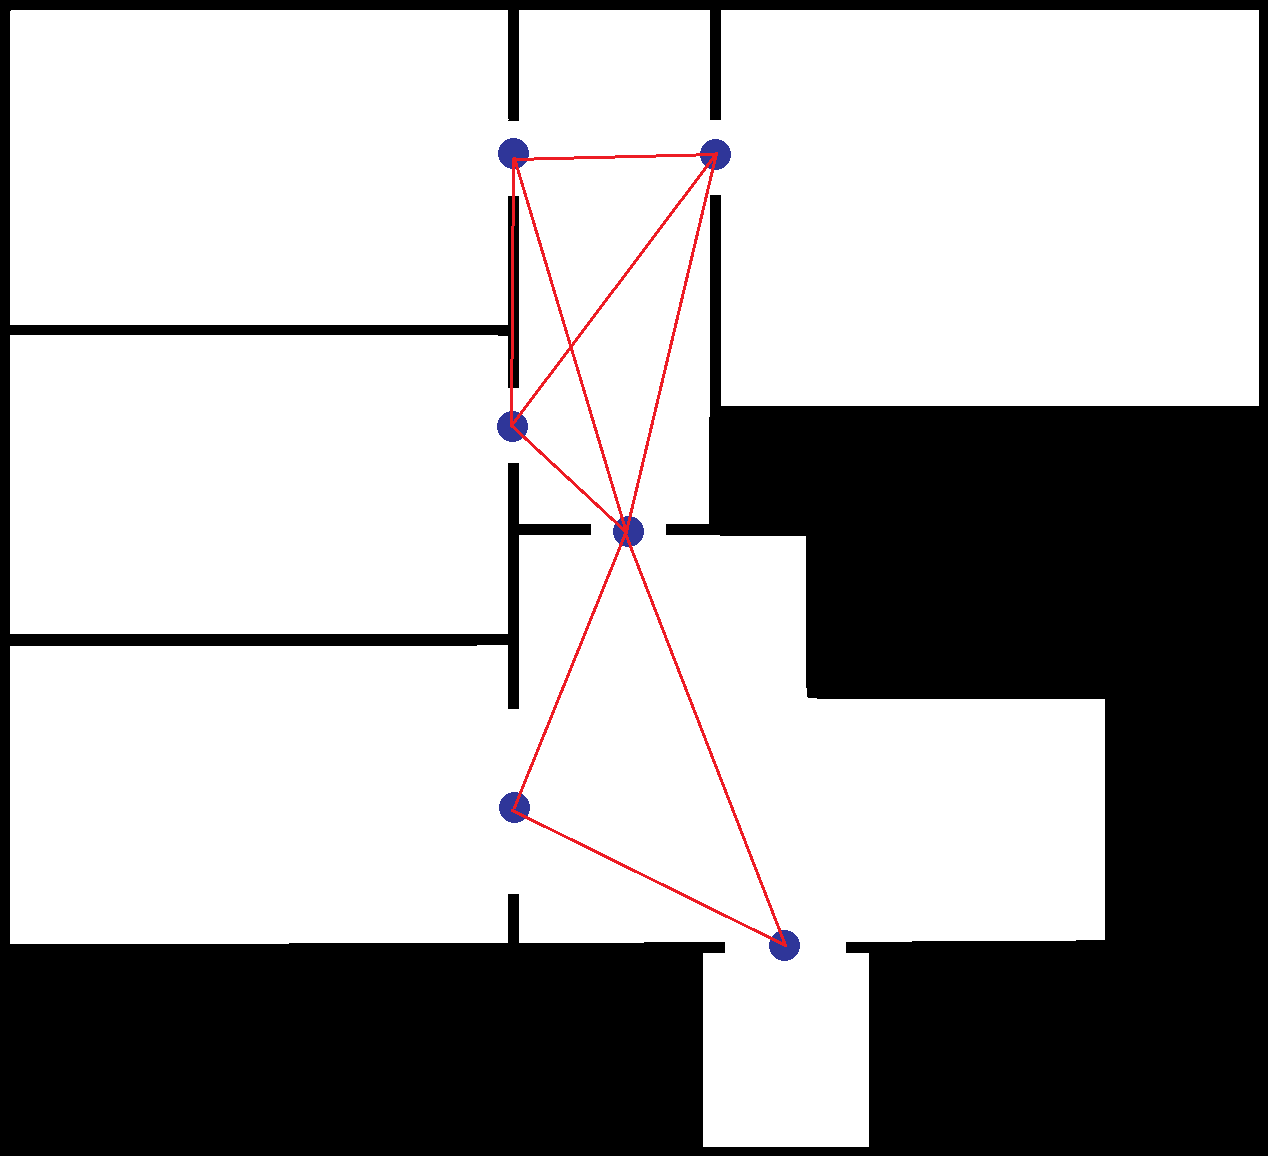
\includegraphics[width=0.8\textwidth]{./images/chapter5/graph_on_map_2.png}
         \label{fig:graph_on_map_2}
     \end{subfigure}
     \caption{Παραδείγματα Γράφων πάνω στο OGM}
    \label{fig:graph_on_map_examples}
\end{figure}




\subsection{Υπολογισμός Βέλτιστης Διαδρομής}
\label{subsection:room_sequence_implementation}

Η βέλτιστη διαδρομή υπολογίζεται, αρχικά, με τον αλγόριθμο \emph{anneal HC}. Αυτός αποτελεί μια παραλλαγή του vanilla HC στην οποία γίνονται αποδεχτές πιθανοτικά και μεταβολλές της λύσης που δεν βελτιώνουν το τελικό αποτέλεσμα \ref{section:hill_climbing}. Η συνάρτηση βελτιστοποίησης είναι η συνολική απόσταση μιας ολόκληρης κυκλικής διαδρομής. Επισημαίνεται ότι χρησιμοποιείται στο άθροισμα και η απόσταση μεταξύ του τελευταίου κόμβου προς τον πρώτο προκειμένου να βρεθεί μια γενικευμένη λύση η οποία δεν καθορίζεται από την αρχή της διαδρομής. Αυτό δίνει την δυνατότητα στο ρομποτικό όχημα να μπορεί να εκκινήσει από ένα οποιοδήποτε δωμάτιο και να εκτελέσει κυκλικά την διαδρομή μέχρι να τα επισκεφτεί όλα. Άλλωστε είναι θεμιτό να αρχίζει η επίσκεψη των δωματίων με πρώτο το δωμάτιο στο οποίο βρίσκεται αρχικά το όχημα.

Η υλοποίηση του αλγορίθμου βασίστηκε σε μια ήδη υπάρχουσα υλοποίηση \cite{tspHC} και παρουσιάζεται στο \ref{alg:anneal}. Περιέχει τόσο την βάση της HC μεθόδου, που μεταβάλλει την λύση προς τα καλύτερα αποτελέσματα, όσο και την στοχαστικότητα της anneal τεχνικής. Αναλυτικότερα, η τιμή $T$ επιλέγεται στο 1.0 και η τιμή $alpha$ στο 0.95. Η καλύτερη λύση $best$ αρχικοποιείται ως ο αύξων δείκτης των κόμβων και υπολογίζεται το κόστος της $best\_score$. Για κάθε βέλτιστη λύση υπολογίζονται όλοι οι πιθανοί συνδιασμοί αντιστροφής τμημάτων της. Για παράδειγμα στην αλληλουχία 1-2-3-4-5-6-7-8 δύο πιθανές αντιστροφές επιφέρουν τις εξής ακολουθίες 1-2-5-4-3-6-7-8 και 1-2-3-4-8-7-6-5. Αυτό έχει ως αποτέλεσμα να μεταβάλλεται η λύση προς κάθε κατεύθυνση και να εξετάζεται το κόστος της κάθε πιθανής διαδρομής. Η αποδοχή ή μη της κάθε μεταβολής εξαρτάται από τον πιθανοτικό παράγοντα $p$ ο οποίος εισάγει την στοχαστικότητα στον αλγόριθμο αυτό μέσω της τιμής $T$. Αφότου εξεταστούν όλες οι πιθανές μεταβολές της αλληλουχίας ή βρεθεί κάποια νέα καλύτερη σειρά, η τιμή $T$ μειώνεται ποσοστιαία κατά $1 - alpha$, έτσι ώστε με την πάροδο των επαναλήψεων να γίνονται δεκτές όλο και λιγότερες λύσεις που δυσχεραίνουν το κόστος της διαδρομής. Επιπλέον, η συνολική διαδικασία τερματίζεται είτε όταν συμπληρωθούν οι επαναλήψεις που ορίστηκαν στην μεταβλητή εισόδου $iterations$ είτε εαν καμία μεταβολή της λύσης δεν επιλεγεί αντί της τρέχουσας βέλιστης πράγμα που σημαίνει ότι ο αλγόριθμος έφτασε σε τοπικό ελάχιστο. Τέλος, επιστέφονται η βέλτιστη διαδρομή, το κόστος της και το πλήθος των επαναλήψεων που χρειάστηκαν. 

\newpage

\begin{algorithm}[H]
\caption{Anneal Hill Climb}
\label{alg:anneal}
\begin{algorithmic}[1]
    \Function{anneal}{distances, iterations, start\_temp, alpha}
        \State $length = distances.shape[0]$
        \State $best = range(length)$
        \State Set $best\_score$ equal to the length of route $best$
        \State $iter = 0$
        \State $done = False$
        \State $T = start\_temp$
        \While{not $done$}
            \State Find all possible reversed sections of current route $best$ 
            \State $move\_made = False$
            \For{each reversed route $next$}
                \If{$iter >= iterations$}
                    \State $done = True$
                    \State Break
                \EndIf
                \State Compute length of $next$ route and set it to $next\_score$
                \State $iter += 1$
                \If{$next\_score > best\_score$}
                    \State $p = 1$
                \Else
                    \State $p = math.exp(-abs(next\_score - prev\_score)/T)$
                \EndIf
                \State \Comment{probablistically accept this solution}
                \If{$random.random() < p$}
                    \State $best = next$
                    \State $best\_score = next\_score$
                    \State $move\_made = True$
                    \State $break$
                \EndIf
            \EndFor
            \State $T = T * alpha$
            \If{not $move\_made$}
                \State Break
            \EndIf
        \EndWhile
        \State \Return $door\_route$, $cost$, $iter$
\end{algorithmic}
\end{algorithm}


Μετά υλοποιείται ο \emph{RRHC} αλγόριθμος. Η ανάπτυξη του βασίστηκε και αυτή στην υλοποίση του \cite{tspHC}. Αυτός καλεί τον απλό HC μέχρι αυτός να φτάσει σε ένα τοπικό μέγιστο και κρατάει τη λύση του ως τελική λύση. Στη συνέχεια, επανεκκινεί τη διαδικασία μέχρι να συμπληρωθεί το πλήθος των επαναλήψεων που έχει οριστεί εξαρχής. Φυσικά, κάθε νέο τοπικό μέγιστο που αποτελεί βελτίωση του τρέχοντος καλύτερου, το αντικαθιστά. Ο RRHC αναλύεται στο \ref{alg:rrhc}.


\begin{algorithm}[H]
\caption{Random Restard Hill Climb}
\label{alg:rrhc}
\begin{algorithmic}[1]
    \Function{randomRestartHillClimb}{distances, epochs, fixed\_edges = False}
        \State $best = $ None, $best\_score = 0$, $iter = 0$
        \While{$iter < epochs$}
            \State $iters\_left = epochs - iter$
            \State $sequence, score, iters\_made = hillClimb(distances, iters\_left, fixed\_edges)$
            \State $iter += iters\_made$
            \If{$score < best\_score$ or $best$ is None}
                \State $best\_score = score$, $best = sequence$
            \EndIf
        \EndWhile
        \State \Return $best, best\_score, iter$
\end{algorithmic}
\end{algorithm}


\begin{algorithm}[H]
\caption{Hill Climb}
\label{alg:hc}
\begin{algorithmic}[1]
    \Function{HillClimb}{distances, epochs, fixed\_edges = False}
        \State $length = distances.shape[0]$
        \State $best = range(length)$
        \State Set $best\_score$ equal to the length of route $best$
        \State $iter = 1$
        
        \While{$iter < epochs$}
            \State $move\_made = $ False
            \For{each reversed route $next$}
                \If{$iter >= epochs$}
                    \State break
                \EndIf
                \State Set $next\_score$ equal to the length of route $next$
                \State $iter++$
                \If{$next\_score < best\_score$}
                    \State $best = next$, $best\_score = next\_score$, $move\_made = $ True
                    \State break
                \EndIf
            \EndFor
            \If{not $move\_made$}
                \State break
            \EndIf
        \EndWhile
        \State \Return $best, best\_score, iter$
\end{algorithmic}
\end{algorithm}




\subsection{Aντιστοιχία Κόμβων με Δωμάτια}
\label{subsection:doors_rooms_correspondense}

Ένα απλό αλλά σημαντικό βήμα είναι η αντιστοιχία των κόμβων σε δωμάτια. Η αλληλουχία που έχει υπολογιστεί αφορά τις πόρτες του χώρου, όμως το όχημα χρειάζεται να καλύψει τα διάφορα δωμάτια. Έτσι, δημιουργείται η αλληλουχία δωματίων που προκύπτει από τις πόρτες παίρνοντας για κάθε μία τα δύο δωμάτια που διαχωρίζει, το αριστερό και το δεξί με αυτή την σειρά, δίχως αυτή η θεώρηση να επηρεάζει συνολικά, αφού και τα δύο δωμάτια θα προσπελαστούν. Φυσικά, κάθε φορά ελέγχεται η περίπτωση ένα δωμάτιο να υπάρχει ήδη στην αλληλουχία από μια προηγούμενη πόρτα.


\subsection{Υπολογισμός Πόρτας Εισόδου και Εξόδου}
\label{subsection:enterin_leaving_door_implementation}

Στο τελευταίο βήμα εντοπίζονται οι πόρτες από τις οποίες το όχημα εισέρχεται σε κάθε δωμάτιο και αυτές από τις οποίες εξέρχεται. Αυτό επιτυγχάνεται προσομοιώνοντας την διαδικασία επίσκεψης των διάφορων δωματίων με την σειρά που έχει υπολογιστεί. Χρησιμοποιείται ο γράφος που έχει δημιουργηθεί στο πρώτο βήμα της μελέτης αυτής, καθώς ουσιαστικά κάθε δωμάτιο αποτελεί τις ακμές του γράφου αυτού. Έτσι, ελέγχονται οι κόμβοι που προσπελάσσονται πριν και μετά από την επίσκεψη των ακμών αυτών. Ο αλγόριθμος παρουσιάζεται στο \ref{alg:find_entering_leaving_doors}.

Ο τελικός αλγόριθμος της ενότητας αυτής παρουσιάζεται στην συνέχεια στο \ref{alg:find_room_sequence}. Εδώ παρουσιάζεται η περίπτωση της χρήσης του RRHC, ωστόσο για την χρήση του anneal αλγορίθμου απαιτείται αλλαγή μόνο στην 7η εντολή, χρησιμοποιώντας την εντολή:

$door\_route, cost, iter = anneal(distances, max\_iterations, 1.0, 0.95)$


\begin{algorithm}[H]
\caption{Find Room Sequence}
\label{alg:find_room_sequence}
\begin{algorithmic}[1]
    \Function{findRoomSequence}{door\_nodes, room\_doors}
        \State $room\_sequence = []$
        \State $doors\_length = len(door\_nodes)$
        \If{$doors\_length >= 2$}
            \State $distances, graph = computeDoorDistances(door\_nodes, room\_doors)$
            \State $max\_iterations = 500 * doors\_length$
            \State $door\_route, cost, iter = rrhc(distances, max\_iterations)$
        \Else
            \State $door\_route = [0]$
        \EndIf
        \State \Comment{Correspond door route to room route}
        \For{each $door$ in $door\_route$}
            \For{$i$ in $range(len(room\_doors))$}
                \If{$door\_nodes[door]$ in $room\_doors[i]$ and $i$ not in $room\_sequence$}
                    \State $room\_sequence.append(i)$
                \EndIf
            \EndFor
        \EndFor
        \State $enter, leave = findEnteringLeavingDoors(graph, room\_sequence,$
        \Statex $room\_doors, door\_route)$ 
    \State \Return $room\_sequence, enter, leave$
\end{algorithmic}
\end{algorithm}


\begin{algorithm}[H]
\caption{Find Entering Leaving Doors}
\label{alg:find_entering_leaving_doors}
\begin{algorithmic}[1]
    \Function{findEnteringLeavingDoors}{graph, room\_sequence, room\_doors, door\_route}
    \State $enter = \{\}$, $leave = \{\}$
    \If{$doors\_length >= 2$}
        \State $room\_i = 1$  \Comment{Start from 2nd room}
        \State $room\_idx = room\_sequence[room\_i]$
        \State $entered = False$
        \For{$i$ in $range(len(door\_route))$}
            \State \Comment{Find path from current to next door}
            \State $door\_idx = door\_route[i]$
            \State $next\_door\_idx = door\_route[(i+1)\%len(door\_route)]$
            \State $path = find\_path(graph, door\_idx, next\_door\_idx)$
            \If{$entered$ and $len(path.nodes) > 1$}
            \Comment{if already inside room, first node of path is already used}
                \State $ii = 1$
            \Else
                \State $ii = 0$
            \EndIf
            \State \Comment{Transverse through path and check for corresponding rooms}
            \While{$ii < len(path.nodes)$}
                \State $node\_idx = path.nodes[ii]$, $door = door\_nodes[node\_idx]$
                \If{$door$ in $room\_doors[room\_idx]$}
                    \If{not $entered$}
                        \State $enter[room\_idx] = door$
                        \State $entered =$ not $entered$
                        \If{$len(room\_doors[room\_idx]) == 1$}
                            \State $ii -= 1$    \Comment{To revisit this door}
                        \EndIf
                    \Else
                        \State $leave[room\_idx] = door$
                        \State $entered = $not  $entered$
                        \State $room\_i += 1$
                        \State $room\_idx = room\_sequence[room\_i\%len(room\_sequence)]$
                        \State $ii -= 1$\Comment{To revisit this door}
                    \EndIf
                \EndIf
                \State $ii += 1$
            \EndWhile
        \EndFor
    \Else
        \For{$i$ in $range(length(room\_sequence))$}
            \State $enter[i] = door\_nodes[0]$, $leave[i] = door\_nodes[0]$
        \EndFor
    \EndIf
    \State \Return $enter, leave$
\end{algorithmic}
\end{algorithm}
